\section{Cold, Aging and Charging}\label{sec:aging}

\paragraph{Stranded charge.} Cold and age strand charge rather than burn it (\cref{fig:stranded_map}a). On the
social feed only the new pack at 25\,$^\circ$C reaches the cut-off (0.4\,\% displayed); all others brown out,
stranding 2.8\,\% (new) and 8.5\,\% (SOH 0.8) at $-10\,^\circ$C and 23.3\,\% at $-20\,^\circ$C and SOH 0.8
(TTE 10.2 instead of 16.6\,h). F4 explains it: $R_0$, which is $3.6\times$ higher at
$-20\,^\circ$C and $1.5\times$ at SOH 0.8 ($r_g=\gamma_Rq_{\mathrm{loss}}$), multiplies the burst, so the safe burst
at $\soc=0.2$ falls from 17.4 to 2.2\,W, while the resistive loss stays below 6\,\% (F3). The charge returns
once the phone warms up \cite{LEE20,AP-TEMP}, as in real phones that shut down at 15--35\,\% below 0\,$^\circ$C
(V7, \cref{sec:validation}; magnitudes indicative). The 30\,s, 4.1\,W photo bursts of the cold hike S9 exceed the
cut-off power with $R_0+R_1$ (3.2\,W at mid-charge, $-20\,^\circ$C, SOH 0.8); as the polarization builds up within
a burst the voltage reaches the cut-off (F4). The hike then ends with 44.2\,\% displayed at $-20\,^\circ$C and SOH
0.8 (22.2\,\% at $-10\,^\circ$C), 16.9 and 7.2\,\% on a new pack, and 1.7--2.7\,\% at 25\,$^\circ$C.

\begin{figure}[b]
  \centering
  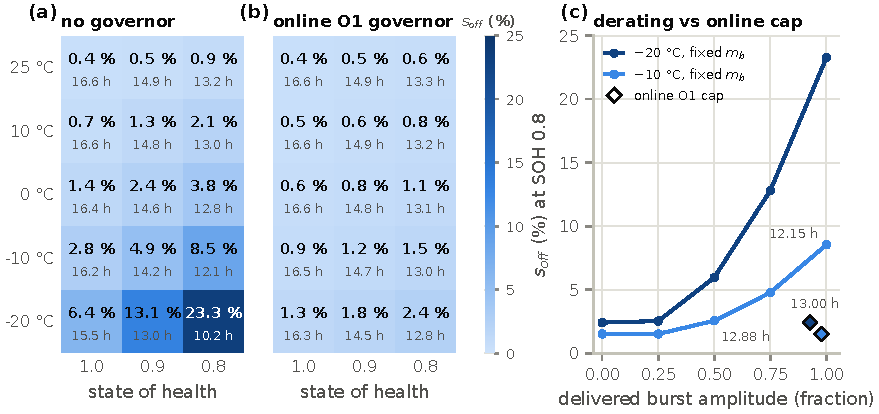
\includegraphics[width=0.76\textwidth]{figures/fig_stranded_map.pdf}
  \caption{Cold-soaked social feed. (a) Displayed SOC at shutdown (bold) and TTE (h). (b) With the peak-power
  governor O1 (\cref{sec:recs}). (c) SOH 0.8: fixed burst derating $m_b$ vs.\ the online cap (diamonds); numbers:
  TTE.}
  \label{fig:stranded_map}
\end{figure}

\begin{figure}[t]
  \centering
  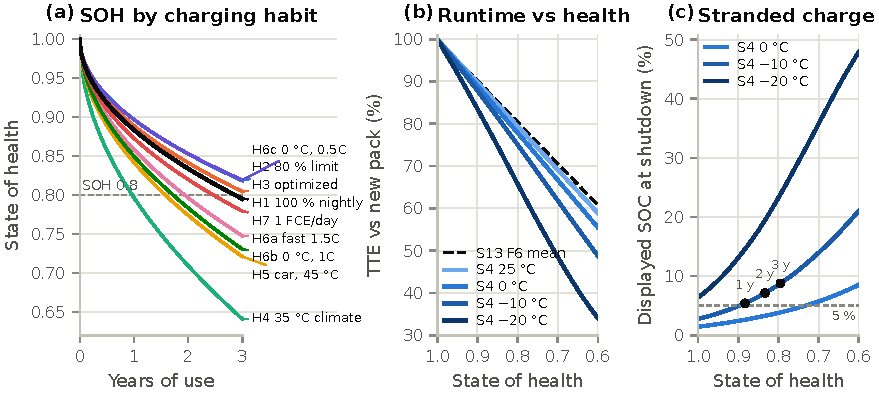
\includegraphics[width=0.77\textwidth]{figures/fig_aging.pdf}
  \caption{(a) SOH for the charging habits H1--H7. (b) TTE relative to a new pack; dashed: F6 mean of the typical
  random day (capacity loss only). (c) Stranded charge of the cold-soaked social feed; dots: H1 after 1, 2, 3
  years; dashed: 5\,\%.}
  \label{fig:aging}
\end{figure}

\paragraph{Charging habits.} The aging layer runs day by day (a typical day's drain, charging overnight at
$\Tamb+8$\,K) and is calibrated to SOH 0.80 after 1000 full cycles \cite{AP-BATT,GOOG}. The baseline habit H1
(100\,\%, held overnight) has SOH 0.834 after two years and 0.8 after 2.86 years (\cref{fig:aging}a). Calendar
loss is the largest single term after two years (0.080, against 0.074 for SEI cycling and 0.013 for plating), and
the habit comparisons below show that heat and a held full charge matter more than extra cycling. After two
years, against H1, a 35\,$^\circ$C climate (H4) costs 12.4 points of SOH (0.8 within 0.96 years), 2\,h a day on a
45\,$^\circ$C car dashboard (H5) 6.0, charging at 1C in a 0\,$^\circ$C room (H6b) 5.0, fast charging at 1.5C (H6a)
3.7 and a full cycle per day (H7) 1.4. An 80\,\% limit (H2) gains 1.9 points and optimized charging (H3)
\cite{AP-OBC,SAM} 0.76; the JEITA rule \cite{TI-JEITA} of charging at 0.5C in the cold (H6c) gains 7.0 over H6b.

\paragraph{Two channels and winter shutdowns.} Capacity loss and resistance growth multiply (\cref{fig:aging}b).
At 25\,$^\circ$C and SOH 0.8 the resistance channel costs 0.7\,\%
($\TTE\approx\TTE_{\mathrm{new}}(1-q)(1-\alpha\gamma_RqP)$ gives 0.797 of the new-pack TTE; L2 0.794); at
$-10\,^\circ$C it costs 6.1\,\% (capacity alone 0.800, resistance alone 0.939, both 0.751) and causes all the
extra stranded charge (2.8\,\% with capacity loss only, 8.5\,\% with both). Two years of H1 shorten the F6 mean of
the typical random day from 41.2 to 34.5\,h (capacity channel only). Taking $\ge5\,\%$ displayed at shutdown as an
illustrative winter-shutdown level, a new pack reaches it at $-20\,^\circ$C (6.4\,\%) and an aged one at
$-10\,^\circ$C at SOH 0.898 (\cref{fig:aging}c): after 0.77 years under H1, 0.98 with the 80\,\% limit, 0.42 with
the car dashboard and 0.26 in a hot climate: hot summers cause winter shutdowns.

\paragraph{Robustness.} In 128 joint samples of ten aging factors, each recalibrated, H2 and H3 beat H1 in every
sample (90\,\%: $+0.4$ to $+2.9$ and $+0.05$ to $+1.3$ points) and H4, H5, H6a and H7 lose in all. The
plating rate sensitivity $\beta_L$ is sourced only at its upper end (LFP, i.e.\ LiFePO$_4$ cells \cite{SCM18}); at
$\beta_L=0.5$ fast charging costs almost nothing (H6a 0.830 vs.\ H1 0.833 at two years) and H6c falls behind H1
(0.799), while the 0\,$^\circ$C-charging penalty stays (H6b 0.780).
